%%%%%%%%%%%%%%%%%%%%%%%%%%%%%%%%%%%%%%%%%%%%%%%%%%%%%%%%%%%%%%%%%%%%%%%%%%%%%%%%%%%%%%%%%
%%                                                                                     %%
%%                This file is part of the CAPH Compiler distribution                  %%
%%                            http:%/caph.univ-bpclermont.fr                           %%
%%                                                                                     %%
%%                                  Jocelyn SEROT                                      %%
%%                         Jocelyn.Serot@univ-bpclermont.fr                            %%
%%                                                                                     %%
%%         Copyright 2011-2018 Jocelyn SEROT.  All rights reserved.                    %%
%%  This file is distributed under the terms of the GNU Library General Public License %%
%%      with the special exception on linking described in file ..%LICENSE.            %%
%%                                                                                     %%
%%%%%%%%%%%%%%%%%%%%%%%%%%%%%%%%%%%%%%%%%%%%%%%%%%%%%%%%%%%%%%%%%%%%%%%%%%%%%%%%%%%%%%%%%

\chapter{Dealing with images}
\label{cha:lang-images}

In this chapter we will show how to use CAPH to implement a very simple image processing application.
This will be the opportunity to introduce the core concepts used for dealing with images -- mainly
their representation as \emph{structured streams} of pixels -- and to describe the tools used for
manipulating them at the simulation level.

\section{Representation of images}
\label{sec:repr-imag}

In chapter~\ref{cha:lang-basic}, the dataflow network used as an example, was operating on a raw,
unstructured stream of data. In contrast, images are \emph{structured} streams of pixels. In
particular, in most of applications, we need a way to encode the dimensions of a given image (so
that we can tell, for example, if a stream of 64 pixels actually represents an image with 8 lines of
8 pixels, an image with 4 lines of 16 pixels or even four successive images with 4 lines of 4
pixels).

For this, the idea is to insert, in the stream of pixels, \emph{control} tokens expliciting the
underlying structure of the data and to distinguish control tokens from \emph{data} tokens (carrying
pixel values) by attaching a \emph{tag} to each token. In practice, for an application having to
process images, the input of will be a sequential stream of tokens, where each
single token is either
\begin{itemize}
\item the tag \verb|SoI| (start of image),
\item the tag \verb|EoI| (end of image),
\item the tag \verb|SoL| (start of line),
\item the tag \verb|EoL| (end of line),
\item a pixel value, with tag \verb|Pixel|.
\end{itemize}

With this scheme, the $4 \times 4$ image depicted in Fig.~\ref{fig:img4}, for example, will be
represented (``encoded'') by the following stream of tokens:

%\footnotesize
\begin{center}
\begin{spverbatim}
SoI SoL Pixel(10) Pixel(30) Pixel(55) Pixel(90) EoL SoL Pixel(33) Pixel(53)
Pixel(60) Pixel(12) EoL SoL Pixel(99) Pixel(56) Pixel(23) Pixel(11) EoL SoL
Pixel(11) Pixel(82) Pixel(46) Pixel(11) EoL  EoI
\end{spverbatim}
\end{center}
%\normalsize

\begin{figure}[h]
  \centering
  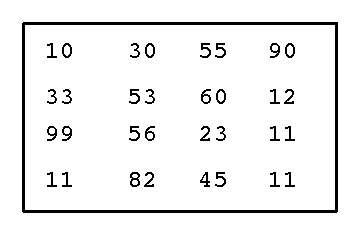
\includegraphics[width=0.25\linewidth]{figs/img4}
  \caption{A $4 \times 4$ image}
  \label{fig:img4}
\end{figure}

In fact, only two distinct control tokens are needed :

\begin{itemize}
\item a token \verb|SoS| (\emph{start of structure}), signaling the start of an image or the start
  of a line within a image,
\item a token \verb|EoS| (\emph{end of structure}), signaling the end of an image or the end
  of a line within a image.
\end{itemize}

As a result, and using the following abbreviations :
\begin{itemize}
\item \verb|<| for \verb|SoS|,
\item \verb|>| for \verb|Eos|,
\item \verb|v| for \verb|Pixel(v)|,
\end{itemize}

the image depicted in Fig.~\ref{fig:img4}, can be represented by the following stream of tokens~:

%\footnotesize
\begin{center}
\begin{spverbatim}
< < 10 30 55 90 > < 33 53 60 12 > < 99 56 23 11 > < 11 82 46 11 > >
\end{spverbatim}
\end{center}
%\normalsize

\section{Processing images}
\label{sec:processing-images}

By using the pattern-matching mechanism introduced in Chap.~\ref{cha:lang-basic} it is
very easy to describe the behavior of actors operating on structured streams of values. 

\medskip
Consider, for example, an actor performing image negation on images made of 8-bit unsigned pixels,
\emph{i.e.} each pixel having value $v$ is transformed to a pixel having value $255-v$. 

Such an actor is decribed in Listing~\ref{lst:inv-actor}. 

First, note that the type of the input and output for this actor (\verb|i| and \verb|o|, lines 2--3)
is \emph{not}

\begin{center}
\verb|unsigned<8>|
\end{center}

but

\begin{center}
\verb|unsigned<8> dc|
\end{center}

 The type \verb|dc| (abbreviation for \emph{data or
  control}) is here used for representing structured values\footnote{CAPH uses so-called
  \emph{algebraic data types} (aka \emph{variant types}) for this. Internally, the \texttt{dc} type
  constructor is defined as : 

\texttt{type \$t dc = SoS | EoS | Data of \$t}

where \texttt{SoS}, \texttt{EoS} and \texttt{Data} are the \emph{value
  constructors} associated to tags and $\$t$ denotes a \emph{type variable}. The notations
\texttt{'<}, \texttt{'>} and \texttt{'v} are then abbreviations for \texttt{SoS}, \texttt{EoS} and
\texttt{Data v} respectively.}.
A value having type \verb|t dc|, where
\verb|t| is a scalar (unstructured) type, is either
\begin{itemize}
\item the control value \verb|SoS| (which can be abbreviated as \verb|'<|),
\item the control value \verb|EoS| (which can be abbreviated as \verb|'>|),
\item a data value \verb|v|, of type \verb|t| (which can be abbreviated as \verb|'v|).
\end{itemize}

The actor rules use the pattern matching mechanism to inspect the tag of
the input value and to produce the appropriate value on output :
\begin{itemize}
\item if the input token is a control token (\verb|'<| or \verb|'>|, lines 5 or 6), write the same token on output
  (this means that the \emph{structure} of the image is unchanged),
\item if the input token is data token (pixel), carrying value \verb|x| (line 7), write a data token
  carrying value \verb|255-x| on output.
\end{itemize}

\begin{lstlisting}[style=CaphStyle,numbers=left,numberstyle=\tiny,caption={An actor computing image negatives in
    CAPH},label={lst:inv-actor}]
actor inv
  in (i: unsigned<8> dc)
 out (o: unsigned<8> dc)
rules
| i:'< -> o:'<;
| i:'> -> o:'>;
| i:'x -> o:'255-x;
\end{lstlisting}

\medskip
\textbf{Note 1}. The code in Listing~\ref{lst:inv-actor} uses the abbreviated syntax for denoting
values with type \verb|unsigned<8> dc|. It is also possible to use the un-abbreviated syntax, as
shown in Listing.~\ref{lst:inv-actor2}. 

\begin{lstlisting}[style=CaphStyle,caption={An actor computing image negatives in
    CAPH (alternate syntax)},label={lst:inv-actor2}]
actor inv
  in (i: unsigned<8> dc)
 out (o: unsigned<8> dc)
rules
| i:SoS -> o:SoS;
| i:EoS -> o:EoS;
| i:Data(x) -> o:Data(255-x);
\end{lstlisting}

\medskip
\textbf{Note 2}. The CAPH type system ensures that tagged and untagged values are used consistently
in programs. It we write, for example, the last rule of actor \verb|inv| as :

\begin{lstlisting}[style=CaphStyle]
| i:x -> o:255-x;
\end{lstlisting}

we get the following error message from the compiler :

\begin{lstlisting}[style=BashOutputStyle]
File "inv.cph", line 7, characters 11-16:
>| i:x -> o:255-x;
>...........^^^^^
An error occured when typing this expression: types unsigned<#a> and unsigned<8> dc cannot be unified.
\end{lstlisting}

What the type checker detects here is that the output \verb|o|, supposed to have type
\verb|unsigned<8> dc| (\emph{i.e.} to be assigned a tagged value) is actually assigned a value of
type \verb|unsigned<n>|\footnote{The notation \texttt{\#a} designates a \emph{size variable}. It
  basically means "any, unknown, size n".} (\emph{i.e.} the untagged value $255-x$). 

\bigskip
In chapter~\ref{cha:cl-images}, we will describe the implementation, simulation and synthesis of an
application making use of the \verb|inv| actor.


%%% Local Variables: 
%%% mode: latex
%%% TeX-master: "caph-primer"
%%% End: 
